\documentclass[a4paper,11pt]{article}

\renewcommand\thesection{\arabic{section}.}

\usepackage{tocloft}
\cftsetindents{section}{0em}{2em}
\cftsetindents{subsection}{0em}{2em}
\renewcommand\cfttoctitlefont{\hfill\Large\bfseries}
\renewcommand\cftaftertoctitle{\hfill\mbox{}}
\setcounter{tocdepth}{10}

\usepackage{listings}
\usepackage{xcolor}

\usepackage{fullpage}

\usepackage{float}

\usepackage{amsfonts}
\usepackage{fontspec}
\usepackage{newunicodechar}
\newfontface{\freeserif}{FreeSerif}
\newunicodechar{▲}{{\freeserif ▲}}

\usepackage{sectsty}
\sectionfont{\fontsize{14}{15}\selectfont}

\usepackage{graphicx}
\usepackage[margin=0.6in,includefoot,headsep=0.1in]{geometry}
\usepackage{fancyhdr}
\pagestyle{fancy}
\fancyhf{}
\cfoot{\thepage}
\rfoot{P. T. O.}
\lfoot{ROHIT DAS 30000114022}

\usepackage{booktabs}
\usepackage{tabularx}

%\usepackage{array}
%\newcolumntype{P}[1]{>{\centering\arraybackslash}p{#1}}

\lstset { %
    language=C,
    backgroundcolor=\color{black!5}, % set backgroundcolor
    basicstyle=\large,% basic font setting
}

\lstset { %
    language=Java,
    backgroundcolor=\color{black!5}, % set backgroundcolor
    basicstyle=\large,% basic font setting
}

\newcommand*{\plogo}{\fbox{$\mathcal{PL}$}} % Generic publisher logo

%----------------------------------------------------------------------------------------
%	TITLE PAGE
%----------------------------------------------------------------------------------------

\newcommand*{\titleGM}{\begingroup % Create the command for including the title page in the document
\hbox{ % Horizontal box
\hspace*{0.18\textwidth} % Whitespace to the left of the title page
\rule{1pt}{\textheight} % Vertical line
\rule{1pt}{\textheight}
\hspace*{0.05\textwidth} % Whitespace between the vertical line and title page text
\parbox[b]{0.75\textwidth}{ % Paragraph box which restricts text to less than the width of the page

{\noindent\Huge\bfseries Software Engineering}\\[2\baselineskip] % Title
{\large \textit{-supervised by:}\\\\\Large \textsc Dr. Suparna Biswas (Saha)}\\[4\baselineskip] % Tagline or further description

{\huge \textsc{Rohit Das}} % Author name
{\\\\\Large{B. Tech(Computer Sc. and Engg)}\\\\\Large{Roll: 30000114022\\\\\Large{Regn. No.:143000110023}\\\\\Large{6th Semester,2016}}}
\vspace{120pt} % Whitespace between the title block and the publisher
\begin{figure}[H]
\hspace*{100pt}
\includegraphics[width=90pt,height=\textheight,keepaspectratio]{/home/mouri/Pictures/makaut.jpg}
\end{figure}
{\noindent \textit{\large{Maulana Abul Kalam Azad University of Technology,\\\\West Bengal.\\\\}}{\large \LaTeX} \hspace{5pt}2017}\\[\baselineskip] % Publisher and logo
}}
\endgroup}

\begin{document}
%\pagestyle{empty} % Removes page numbers
\thispagestyle{empty}
\titleGM % This command includes the title page

\iffalse
\title{\textbf{\Huge Maulana Abul Kalam Azad University of\\[10pt] Technology}}
\date{\vspace{-5ex}}
\maketitle
\begin{center}
\textbf{\LARGE{(SOftware Engineering Assignment)}}
\end{center}
\begin{figure}[H]
\centering
\includegraphics[width=350pt,height=\textheight,keepaspectratio]{/home/mouri/Pictures/makaut.jpg}
\end{figure}
.

\begin{flushright}
\underline{\textbf{\author{\Huge Rohit Das}}}\\
\textbf{\LARGE{
B. Tech(CSE),5th Year\\
Roll No.: 3000114022\\
Regn. No.: 143000110023\\
Taught by: Dr .Suparna Biswas (Saha)\\
}}
\end{flushright}
%\tableofcontents
%\begin{table}[htbp]
%\centering
\fi

\tableofcontents
\break

\section{Assignment-1: C programming (Date: 27/10/2017)}
\subsection{Write a program to implement Calendar program to display Day of the month. Program will accept year, month and date from user and will display the day of the month.}
\underline{Program:}
\lstinputlisting[showstringspaces=false]{../assign1/1.c}
Output:
\begin{figure}[H]
\centering
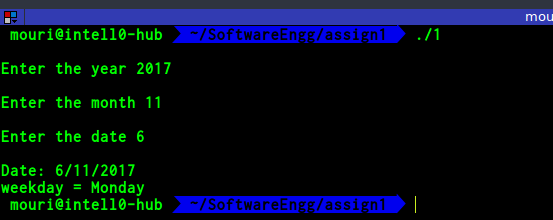
\includegraphics[width=350pt,height=\textheight,keepaspectratio]{./pics/C/1.png}
\end{figure}

\bigskip

%\section{Date: 21/4/2017}
\subsection{Write a program to find inverse of 3x3 matrix.}
\underline{Program:}
\lstinputlisting[showstringspaces=false]{../assign1/2.c}
Output:
\begin{figure}[H]
\centering
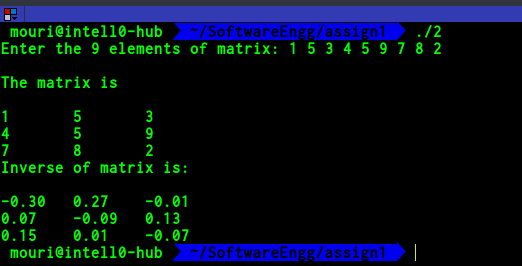
\includegraphics[width=350pt,height=\textheight,keepaspectratio]{./pics/C/2.png}
\end{figure}

\bigskip

%\section{Date: 28/4/2017}
\subsection{Write a program to check whether matrix is Magic Square or not.}
\underline{Program:}
\lstinputlisting[showstringspaces=false]{../assign1/3.c}
Output:
\begin{figure}[H]
\centering
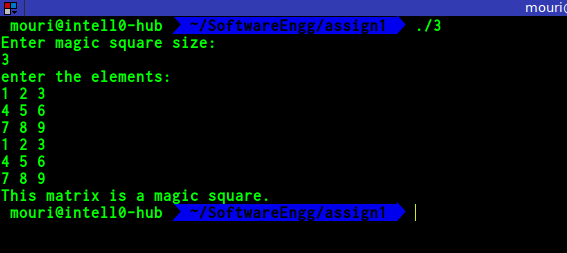
\includegraphics[width=350pt,height=\textheight,keepaspectratio]{./pics/C/3.png}
\end{figure}
\bigskip

\subsection{Write a program to read last n characters from a file(input should be a.txt).}
\underline{Program:}
\lstinputlisting[showstringspaces=false]{../assign1/a.txt}

\lstinputlisting[showstringspaces=false]{../assign1/4.c}
Output:
\begin{figure}[H]
\centering
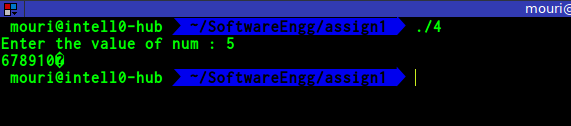
\includegraphics[width=350pt,height=\textheight,keepaspectratio]{./pics/C/4.png}
\end{figure}
\bigskip

%\section{Date: 5/5/2017}
\subsection{Write a program to print binary numbers in pyramid pattern.}
\underline{Program:}
\lstinputlisting[showstringspaces=false]{../assign1/5.c}
Output:
\begin{figure}[H]
\centering
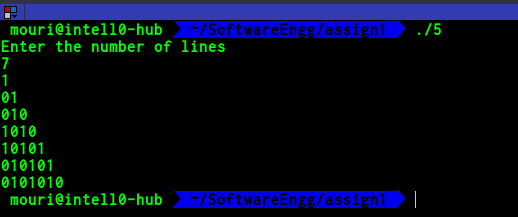
\includegraphics[width=350pt,height=\textheight,keepaspectratio]{./pics/C/5.png}
\end{figure}
\bigskip

%\section{Date: 12/5/2017}
\subsection{Write a program to input password for validation of username.\\
Enter password: ******\\
Password entered: sourav}
\underline{Program:}
\lstinputlisting[showstringspaces=false]{../assign1/6.c}
Output:
\begin{figure}[H]
\centering
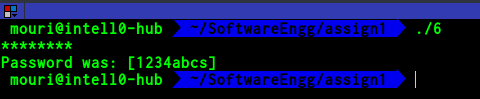
\includegraphics[width=350pt,height=\textheight,keepaspectratio]{./pics/C/6.png}
\end{figure}
\bigskip

%\section{19/5/2017}
\subsection{Write a program to create your own header file in C.}
\underline{Program:}
\lstinputlisting[showstringspaces=false]{../assign1/test.h}

\lstinputlisting[showstringspaces=false]{../assign1/7.c}
Output:
\begin{figure}[H]
\centering
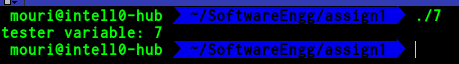
\includegraphics[width=350pt,height=\textheight,keepaspectratio]{./pics/C/7.png}
\end{figure}
\bigskip


\subsection{Write a program to compare two strings without using library function(strcmp).}
\underline{Program:}
\lstinputlisting[showstringspaces=false]{../assign1/8.c}
Output:
\begin{figure}[H]
\centering
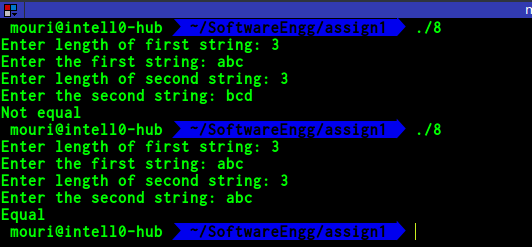
\includegraphics[width=350pt,height=\textheight,keepaspectratio]{./pics/C/8.png}
\end{figure}
\bigskip

\subsection{Write a program to print a rectangle using line and special symbols.}
▲▲▲▲▲▲▲▲▲▲\\
▲ - - - - - - - - - - ▲\\
▲ - - - - - - - - - - ▲\\
▲ - - - - - - - - - - ▲\\
▲ - - - - - - - - - - ▲\\
▲ - - - - - - - - - - ▲\\
▲ - - - - - - - - - - ▲\\
▲▲▲▲▲▲▲▲▲▲\\
\underline{Program:}
\lstinputlisting[showstringspaces=false]{../assign1/9.c}
Output:
\begin{figure}[H]
\centering
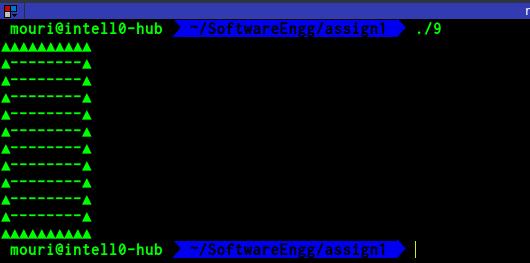
\includegraphics[width=350pt,height=\textheight,keepaspectratio]{./pics/C/9.png}
\end{figure}
\bigskip

\subsection{Write a program to find addition of lower triangular matrix.}
\underline{Program:}
\lstinputlisting[showstringspaces=false]{../assign1/10.c}
Output:
\begin{figure}[H]
\centering
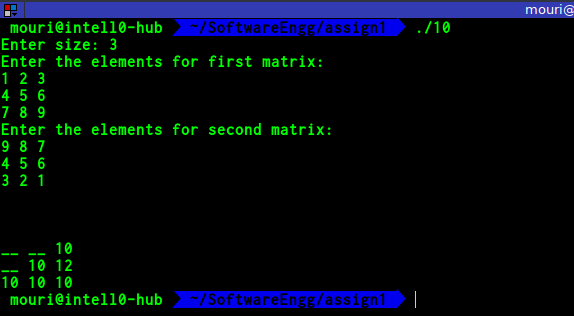
\includegraphics[width=350pt,height=\textheight,keepaspectratio]{./pics/C/10.png}
\end{figure}
\bigskip

\newpage
\section{Assignment-2: Java programming (Date: 30/10/2017)}
\subsection{An array contains 20 integers arranged randomly. Write a Java program using quick sort to sort these numbers in ascending order.}
\underline{Program:}
\lstinputlisting[showstringspaces=false]{../assign2/1.java}
Output:
\begin{figure}[H]
\centering
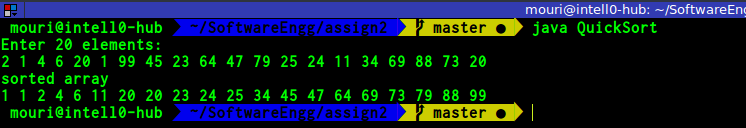
\includegraphics[width=350pt,height=\textheight,keepaspectratio]{./pics/Java/1.png}
\end{figure}

\bigskip

\subsection{Write a Java program to take an integer not greater than 20 as input and calculate the factorial of the integer recursively.}
\underline{Program:}
\lstinputlisting[showstringspaces=false]{../assign2/2.java}
Output:
\begin{figure}[H]
\centering
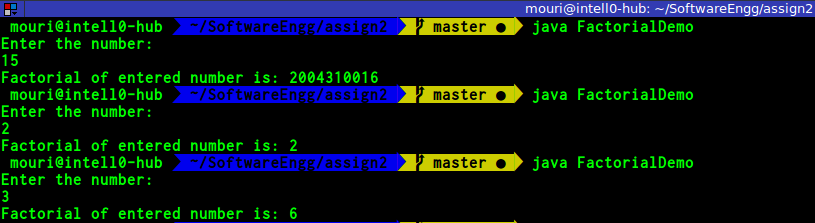
\includegraphics[width=350pt,height=\textheight,keepaspectratio]{./pics/Java/2.png}
\end{figure}

\bigskip

\subsection{You are starting out on a long (really long) trip. On the way, there are N gas stations, the locations of which are given as $a_1,a_2,...,a_N$. Initially you are located at the gas station at $a_1$, and your destination is at location $a_N$.} \textbf{\large Your car can only store enough fuel to travel atmost M units without refilling. You can stop at any station and refill the car by any amount. Now you wish to plan your trip such that the number of intermediate stops needed to reach the destination is minimum, and also how many ways are there to plan your trip accordingly.\\
Input :\\
The first line two space seperated integers N and M. N lines follow, and the ith line has the value $a_i (0 <= a_i <= 1000000000)$. The input will be such that a solution will always exist.\\
Output :\\
Output two space seperated integers : The least number of stops, and the number of ways to plan the trip which uses the least number of stops. Output this value modulo 1000000007.\\}\\
\underline{Program:}
\lstinputlisting[showstringspaces=false]{../assign2/3.java}
Output:
\begin{figure}[H]
\centering
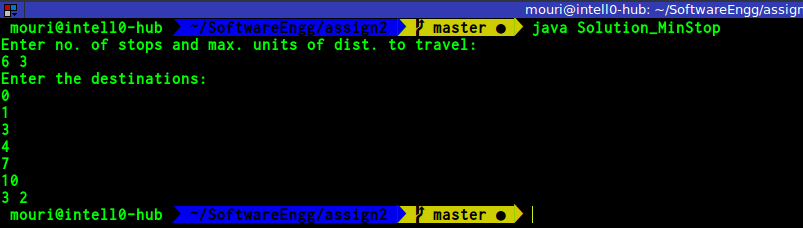
\includegraphics[width=350pt,height=\textheight,keepaspectratio]{./pics/Java/3.png}
\end{figure}

\bigskip

\subsection{Given N separate integer points on the Cartesian plane satisfying: there is no any three of them sharing a same X-coordinate. Your task is to count the number of rectangles (whose edges parrallel to the axes) created from any four of given points.}
\textbf{\large Input:\\
There are several test cases (ten at most), each formed as follows:\\
The first line contains a positive integer N (N ≤ 105).
N lines follow, each containing a pair of integers (each having an absolute value of 109 at most) describing coordinates of a given point. The input is ended with N = 0.\\
Output:\\
For each test case, output on a line an integer which is the respective number of rectangles found.}\\\\
\underline{Program:}
\lstinputlisting[showstringspaces=false]{../assign2/4.java}
Output:
\begin{figure}[H]
\centering
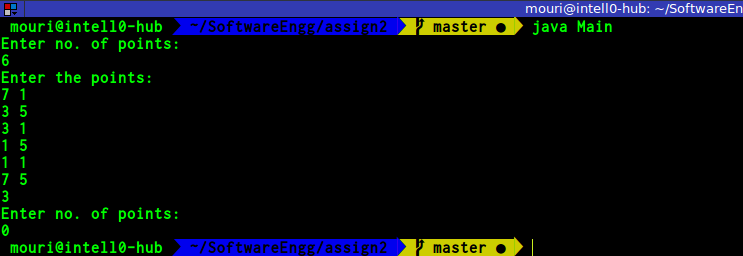
\includegraphics[width=350pt,height=\textheight,keepaspectratio]{./pics/Java/4.png}
\end{figure}

\bigskip

\subsection{Given two strings, write a program that outputs the shortest sequence of character insertions and deletions that turn one string into another.}
\underline{Program:}
\lstinputlisting[showstringspaces=false]{../assign2/5.java}
Output:
\begin{figure}[H]
\centering
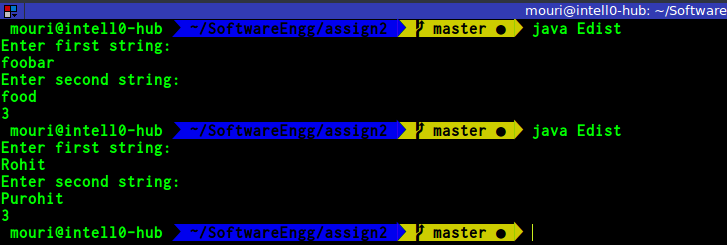
\includegraphics[width=350pt,height=\textheight,keepaspectratio]{./pics/Java/5.png}
\end{figure}

\bigskip

\subsection{Write a java program to generate a 3x3 magic square matrix, where a magic square is a matrix whose all numbers along every row, column and diagonal add up to the same number.}
\underline{Program:}
\lstinputlisting[showstringspaces=false]{../assign2/6.java}
Output:
\begin{figure}[H]
\centering
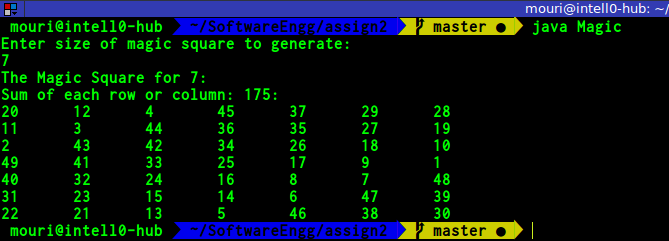
\includegraphics[width=350pt,height=\textheight,keepaspectratio]{./pics/Java/6.png}
\end{figure}

\bigskip

\end{document}